\documentclass{article}
% \usepackage[utf8]{inputenc}
\usepackage[margin=1in]{geometry}
\usepackage{common}
\usepackage{pagesetup}

\begin{document}
%\lecture{**LECTURE-NUMBER**}{**DATE**}{**LECTURER**}{**SCRIBE**}
\lecture{23}{November 29}{Sasha Rush}{Anirudh Suresh, Michael Jasper, Udit Gupta, Donghun Lee}{Applications: Attention and Translation}%% Add your scribe names!!

\subsection{Announcements}

We're going to move December 6 event to be a half hour later and in MD lobby. We have put up instructions for poster printing on the Piazza site. I've been meeting with people with final project questions. I'm going to add some time slots for Friday and Monday to have more time to talk to people and answer any remaining questions.

\subsection{Content}

I'm going to spend first two thirds of class talking about topic relevant to my research. I'll spend last third of class summing up and coming to where we're at in 281.

\subsubsection{Attention}

Attention is less a kind of formally designed thing and more a series of techniques, but much more important than I would have thought 3-4 years ago. Basically, as in many of our lectures this semester, we're gonna talk about the basic probabilistic model. The probabilistic model draws from a Naive Bayes model. In Naive Bayes, we have a latent variable $z$ directed toward a variable $y$, with a set of $k$ different parameters $\mu$ directed to $y$. This is part of that core mixture model idea, with $z$ latent. In practice, we would get a bunch of observations of $y$.\\

This describes for us to how to build clustering model, classification models, how to set up most forms of inference (MCMC, Variational Inference, EM, etc.): core model for our problems of inference. Often, reducing your own problem to a probabilistic framework is good. One of the models often found in NLP is as follows: given several $x$s as input, and a latent variable that chooses a particular $x$, we want to model the $y$s based on \textit{only} the $x$ of importance. What's the probability of each of the $y$s based on the $x$?\\

Let's consider a sequence $x_{1:T} = \{x_1,\ldots,x_T\}$. I have a latent $z$ variable: a selection from $\{1,\ldots,T\}$. Then, my $y$s will only depend on $x_z$. The graphical model below helps to explain this model scheme.

\begin{figure}[h]
    \centering
    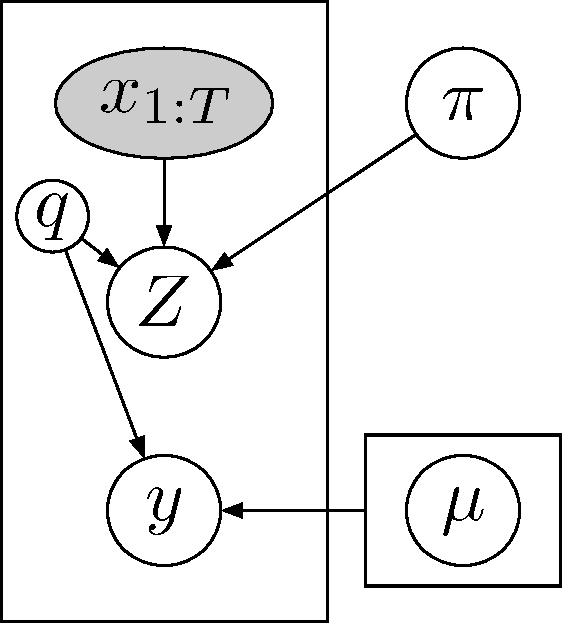
\includegraphics[width=0.25\textwidth]{figs/translation_dgm.pdf}
    \caption{}
    \label{fig:trans_dgm}
\end{figure}

How to choose the latent $z$ will depend on the structure of the environment; prediction of the $y$s is based on the $x$ that is selected.\\

One tangible example of this in the real world is that of Q&A with retrieval: imagine you have a bunch of Wikipedia articles, each about some topic, and you're given some query. You'd like to answer that query, but you want to differentiate meaningful/relevant articles from ones that don't help you answer that query. Given the query $q$ (e.g. Who is the prince of England?), we would like to select an article from $x_{1:T}$ and use that to provide the answer $y$ (e.g. $y = Joe$). Here, $z$ is the selection of the exact Wikipedia page we choose to look at.\\

This is a complicated problem. All sorts of things are going on with respect how you might use the query to select a page and answer the question. The key aspect is given some source of information, how could we possibly perform inference in this model? We know we observe $x$s and we don't know the latent $z$, $\mu$ parameters, etc. Then, we can use an approach from our bag of tricks. For example, we could try EM--1) compute the posterior marginals, 2) computer MLE parameters, 3) repeat until convergence. In this example, this requires an understanding of a distribution over the $z$s (all Wikipedia articles). Depending on which Wikipedia articles help us get the right answer over training data, we can reinforce the probability we choose those articles in future query answers. We could also use Gibbs sampling, VI, or another approach that we've learned this semester.

\subsubsection{Translation}

One of the other problems that uses this type of model is that of machine translation. In machine translation, you want to map a foreign language sentence to a sentence in the native language. Machine translation was developed almost entirely around the source, encoder, noisy channel, decoder analogy of information theory.

\begin{figure}[h]
    \centering
    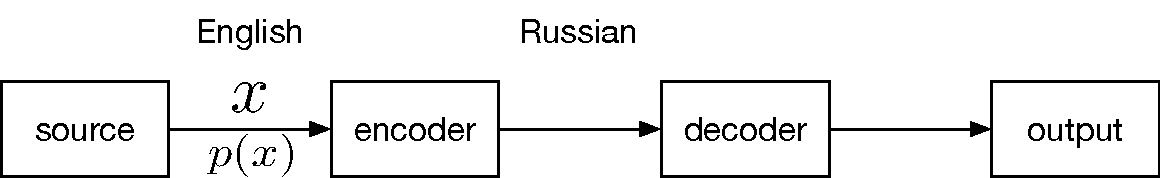
\includegraphics[width=1.0\textwidth]{figs/encoder_translation.pdf}
    \caption{The source, encoder, noisy channel, decoder analogy of information theory.}
    \label{fig:sedo}
\end{figure}

A pioneer of machine translation, Warren Weaver asserted that when someone says something in another language, that can be interpreted simply as a form of English that is severely noised. Source encoding is easy; all we need is a model of English and how likely any sentence is to come out in English. But understanding the encoding step is harder; it's in essence the $p(y \given x)$ part. Given a sentence $x_{1:T}$, we wish to develop a probabilistic model for how it got gargled in another language. We can do that by using the graphical model below.\\

\begin{figure}[h]
    \centering
    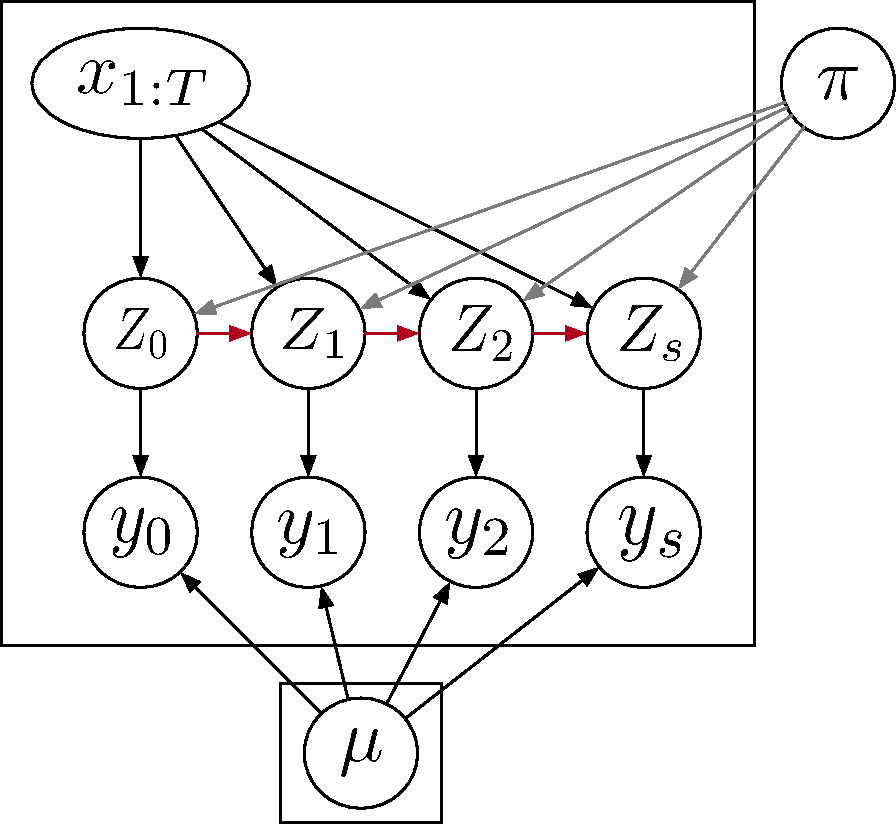
\includegraphics[width=0.40\textwidth]{figs/mt_dgm.pdf}
    \caption{}
    \label{fig:mt_dgm}
\end{figure}

We define $z_j$ to be a one-hot vector, $z_j \in \{0,1\}^T$. The different $z_j$s are selectors that relate to the gargling of different sentences of interest. The $\mu$ here is in essence a dictionary; it provides conditional probabilities that a gargled word/sentence could have come from a certain English word/sentence. We can now do the same thing we did earlier: running some inference algorithm to infer the latent parameters for how gargling takes place.\\

Now what kind of probabilistic issues are there with this example as a generative process? In particular, what does the graphical model tell us about our assumptions? We choose the $z_j$s just based on the $x$s; they don't have any direct relationship between them. Naturally, it makes sense that the order of words in the first sentence should have some effect on the order of words in the second sentence. Each of the $z_j$s could be amended to depend directly on $z_{j-1}$ as in the case of the red lines in the graphical model below.\\

Given a matrix of words, translating from Spanish to French, for instance, we can use the conditional probability structure of the $z_j$s. We will hence end up using a coordinate ascent-type approach called HMM alignment (Vogel 96) that picks mostly elements along the diagonal of the matrix---this algorithm was used a lot in Google Translate, which is often run using EM with HMMs. The conditional distribution $p(y_i \given z_i, x_{z_i})$ yields a probability distribution $\pi$ that has a value for every English word and every foreign word (for every possibility for $x$ and $y$). This ensuing matrix will be really sparse though, so often in practice, a sparse lookup table is used in order to store any English-foreign word pairs that have ever been translated to each other. The problem with this model is its emphasis on a singular word scope. It assumes a one-to-one translation of one English word to one foreign word. However, that's not always the case; one word in English may map to many words in the foreign language, and vice versa.\\

Let's now say we condition now on $\pi$ and $\mu$ and we need to do posterior inference to get $p(z_{1:T} \given y, \mu, \pi, x)$s. So how do we do that? Well, conditioning out everything else, this just becomes a time series model for $z_{1:T}$.\\

\begin{figure}[h]
    \centering
    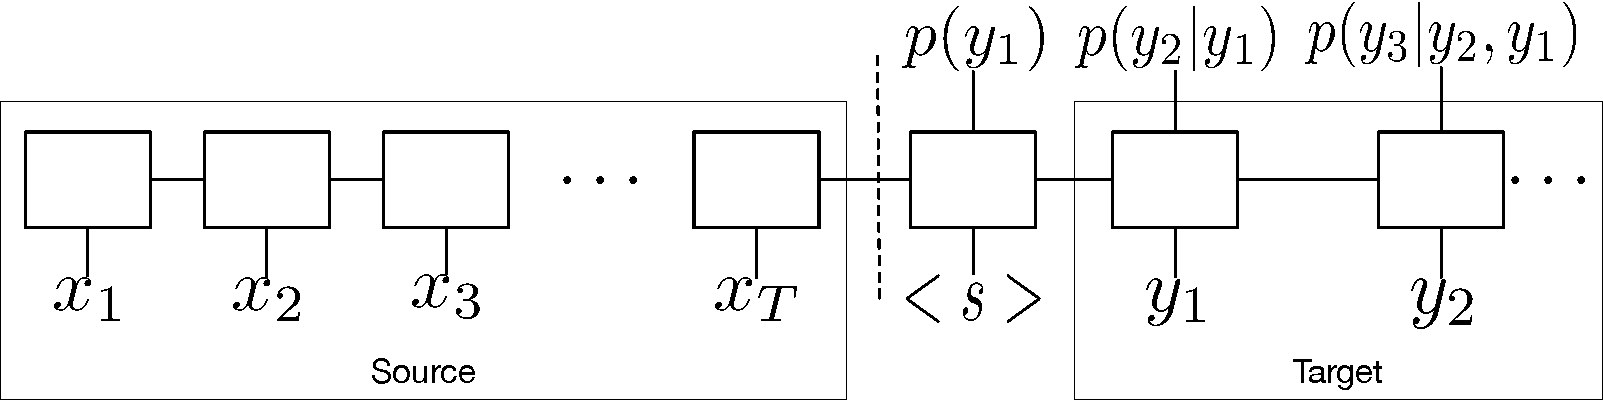
\includegraphics[width=1.0\textwidth]{figs/nn.pdf}
    \caption{Time series model of the problem}
    \label{fig:timeseries}
\end{figure}

Even though we are still in inference mode, we have used conditioning to simplify our model, and now we can use the forward-backward algorithm often used for time series. Recently, there's been movement toward neural nets to model this problem. For example, instead of modeling $p(x)$ by itself, we can model that distribution via an RNN over $x_{1:T}$. The structure of such a model over $x_{1:T}$ is shown below. What people originally tried was to model $p(y \given x)$, the probability of a target sentence given a source sentence. The way people did this was via a version of the above model called a sequence-to-sequence model (https://www.tensorflow.org/versions/r1.1/tutorials/seq2seq).\\

This resembles an RNN over the source, and when you train this, the backpropagation sends weight changes all the way from the predictions for $y_{1:T}$ to the weights of $x_{1:T}$. Thus, the network learns exactly from the prediction errors over the training data. This recurrent neural network is essentially built by stacking over time, and its only probabilistic framework is in the conditional probabilities of $p(y_t \given y_{1:t-1}) \, \forall \, t$. The $x_{1:T}$ layers represent the source, while the $y_{1:T}$ layers represent the target.\\

Then, in the larger picture, what benefits and consequences are there to having explicit latent variables? How is it that this model even works as well as it does in making such transformations? We still don't fully understand all the answers to these questions, but we do know that via an information theory framework we have the maximum amount of information at the middle of this model between the source and target regions; this is essentially a bottleneck.\\

This model came out about 3 years ago, and there was skepticism as to whether this model could do the complicated translations. The hybrid model born out of this model and sequence-to-sequence is the main model in use today. Going back to the Q&A query example, we assume that the latent variable $z_j$ tells us exactly what Wikipedia article we are interested in. What if instead, we said that $p(y \given z, x)$ was of the form $NN(z, x_z)$ where NN denotes Neural Network? Then, instead of picking $z \in \{0,1\}^T$, we picked $z \in \bigtriangleup^T$, a simplex. This means that we pick $z$ to be a convex combination of all the pages in the database. Hence, in the context of our neural network, we take $\mathbb{E}_{z' \sim z \given \mu, q} \big[f(x_z)\big],$ where $f$ is our basis for $x$ and $x_z$ represents the chosen $x$. We can then feed in this entire expectation term into our neural network and use that to predict $y$. In learning, backpropagation is used to train a neural network. If we use expectation here, backpropagation will access the probability distributions of $f$ to access training.\\

To summarize, we take English words and map to an embedding via an RNN; then, we use this embedding to map to words in the foreign language word domain. The main idea of attention networks is that we represent everything in the input via a neural network. After encoding, we use attention to focus on which part of the encoder we wish to focus on upon each prediction. One question is: given $f(x_1), \ldots, f(x_T)$, how might we produce a distribution $p(z \given q, x_{1:T})$? This should certainly be a categorical $Cat(\pi)$, with $\pi_i = f(x_i)^T q$ or $\pi_i = cos(f(x_i)^T q)$ or $\pi_i = \sigma(W'q+W^2f(x_i))$. The weights will then be trained end-to-end via backpropagation in the learning stage of the model.

\subsubsection{Other Applications}

Attention is often applied often to image captioning---the latent $z$ variable is the pixel of an image that is examined closely (\href{https://arxiv.org/abs/1502.03044}{Xu et al 2015}, Figure \ref{fig:show_attend}). It is also often applied to speech recognition (\href{https://arxiv.org/abs/1508.01211}{Chan et al 2015}). A \href{https://www.distill.pub/2016/augmented-rnns/}{cool demo} can be found courtesy of Google Brain. The paper \href{https://arxiv.org/abs/1706.03762}{Attention is All You Need} is a cool paper that applies attention over text (Figure
\ref{fig:attention_need}). Attention is really interesting because it combines a probabilistic framework with the computational side of neural networks.

\begin{figure}[h]
    \centering
    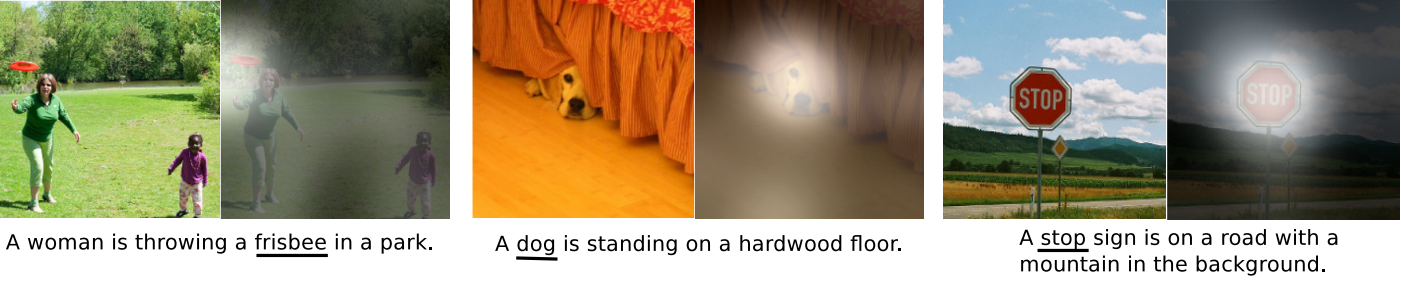
\includegraphics[width=1.0\textwidth]{figs/show-attend-tell.png}
    \caption{Show, Attend and Tell}
    \label{fig:show_attend}
\end{figure}

\begin{figure}[h]
    \centering
    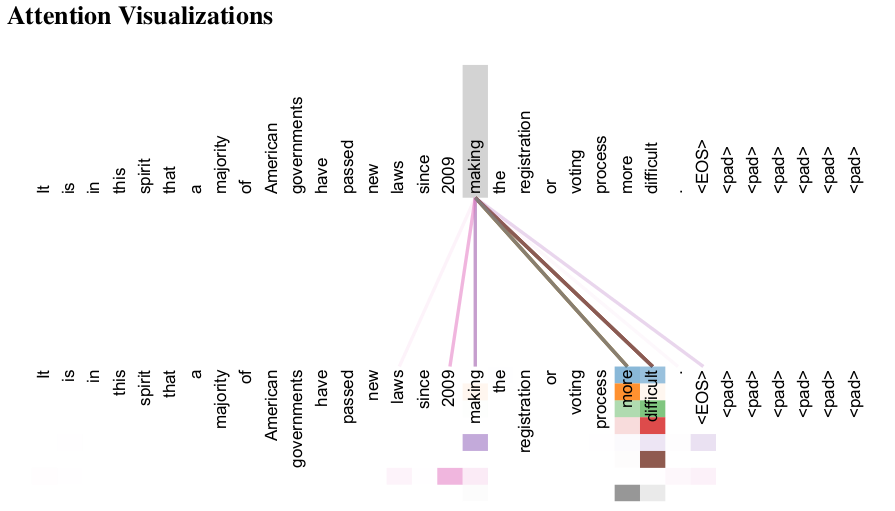
\includegraphics[width=1.0\textwidth]{figs/aaln.png}
    \caption{Attention is All You Need}
    \label{fig:attention_need}
\end{figure}





\subsubsection{Wrapping Up}

Rather than take up too much time to summarize anything from the class, I'm going to spend some time at the front of the lecture hall to talk to any of y'all about your projects and any remaining questions you may have.

\end{document}